\section{Results}
After carrying out the experiments the following results were obtained:

\subsection{Golden Measure}
The average time of execution and the output image subsequent to filtering is shown
below;\\

\textbf{Time taken to filter "small.jpg": 11751.1 ms.}\\

\begin{figure}[!h]
  
\includegraphics[width=\linewidth]{Figures/Output1.jpg}
  \caption{Golden measure Output image}
  \label{fig:boat2}
\end{figure}
As expected, the golden measure, in this case, time of execution for a serial median filter to run
on as a single process. The output image as seen from figure \ref{fig:boat2} has been accuretely
filtered. % is there any other way to validate the filtering of the golden measure?
\subsection{Multi-Threaded Version}
The multi-threaded program aims to optimize the Golden Measure results and uses the quicksort algorithm as mentioned in subsection \ref{sec: threaded}

\subsection{Serial vs Threaded}
The table below shows how the threaded filtering compares to the golden measure by also showing the speed up.
\begin{figure}[!h]
\centering
\begin{tabular}{c|c|c}
Number of threads & Time (ms) & Speed Up\\
\hline
1 & 2243.22 & 5.1708\\
2 & 1161.08 & 9.99\\
4 & 1004.63  & 11.545\\
8 &  996.979 & 11.6344\\
16 &   989.761& 11.72\\
32 & 962.678 & 12.05\\
64 & 845.539 & 13.7\\
128 & 853.736& 13.6\\
\end{tabular}
\caption{Comparison of serial median filtering and threaded filtering}
\end{figure}\\
Figure \ref{fig:boat3} shows how the speed up with using multiple threads with the median filter
compares to the golden measure. The speed up grows very fast between 2 and 8 threads, and then
starts to grow slower from there until with 64 threads where diminishing returns start to appear.\\

However, this approach performs much better that the serial version of the algorithm, we used only
one partitioning scheme across threads, letting thread 1 handle rows 1 to 8, thread 2 rows 9 to 16
etc. \textbf{Why?} Also, the RAM
access stage for each thread need not to go into the critical section because the \dots \\

The correctness of this algorithm however, matches that of the golden measure, we used the
correlation function from Octave to ensure that the filtered pixels are accurate. Correlation gave
a coefficient of 1.
\begin{figure}[!h]
  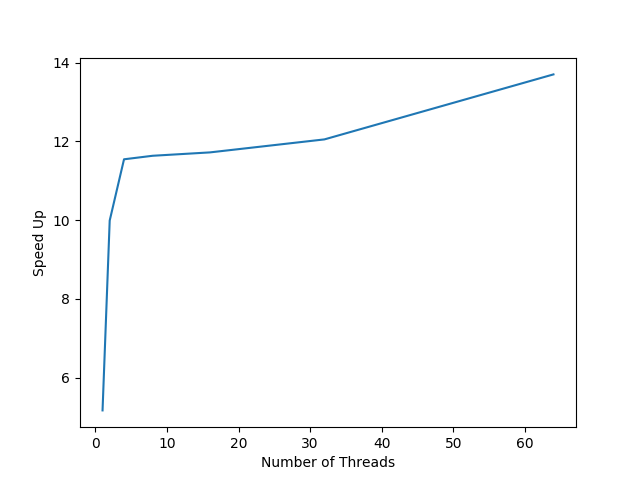
\includegraphics[width=\linewidth]{Figures/speedup.png}
  \caption{Speed up with partitioning the data equally amongst threads (partitioning the rows sequentially)}
  \label{fig:boat3}
\end{figure}


